\chapter*{Introduction}
\addcontentsline{toc}{chapter}{Introduction}
	Ce document a pour objectif de présenter la conception de l'application MyCalendar. Cette application, écrite en C++ avec le framework Qt4, présente une interface graphique correspondant à un emploi du temps semaine par semaine modifiable localement. L'utilisateur peut s'il le souhaite créer, modifier, ou supprimer des évènements.

	Autour de ces fonctionnalités basiques s'attachent deux autres fonctionnalités permettant à l'utilisateur d'intéragir avec certains services en ligne pour importer ou exporter des évènements depuis Internet vers l'application locale et vice-versa.\\

	Petit rappel des spécifications des exigences logicielles à partir desquelles la présente conception est basée :
	\begin{itemize}
		\item Architecture modulaire permettant une maintenance facile de l'application ;
		\item Interface graphique (GUI\footnote{Graphical User Interface}) \emph{user-friendly} par semaine ;
		\item Respect de la charte graphique GNU/Linux ;
		\item Édition locale de l'emploi du temps (ajout, modification, suppression) par clics intuitifs sur la GUI ;
		\item Gestion des conflits (que faire lorsque l'utilisateur essaie d'ajouter un évènement sur un créneau non libre ?) ;
		\item Sauvegarde locale des évènements ;
		\item Exporter l'emploi du temps vers un service en ligne ;
		\item Récupérer l'emploi du temps depuis ce même service en ligne ;
		\item Protection de l'emploi du temps distant avec des identifiants de connexion ;
		\item Utilisation du protocole REST pour la communication avec ce service en ligne ;
		\item Communication non bloquante et temps de réponse de l'ordre de la seconde ;
	\end{itemize}
	\vspace{0.5cm} 
	Une autre exigence est concernée par la conception de l'application puisque nous avons eu le temps de l'implémenter : la récupération d'un emploi du temps universitaire depuis le site de gestion d'emploi du temps de l'Université de Nantes. Cependant, aucun autre format d'emploi du temps n'a été supporté, cette exigence ayant été elle aussi reportée.
		

\chapter{Conception générale}
	%GUILLAUME
	Afin de répondre à la première exigence, c'est-à-dire concevoir l'application à partir d'une architecture modulaire, nous avons utilisé le pattern architectural MVC (pour Model-View-Controller). Cette architecture nous permet de diviser l'application en plusieurs sous-systèmes :
	\begin{enumerate}
		\item L'interface graphique utilisateur ;
		\item Le modèle, contenant tous les évènements et proposant des méthodes pour agir dessus ;
		\item Les interfaces de communication, pour interagir avec différents services d'emploi du temps en ligne ;
	\end{enumerate}
	Le contrôleur joue quant à lui le rôle d'arbitre entre tous ces systèmes.\\
	Exemples :
	
	La vue demande la sauvegarde des évènements dans un fichier local : le contrôleur reçoit le signal correspondant et traite la demande.
	
	La vue demande l'export des évènements vers un service en ligne : le contrôleur reçoit ce signal, vérifie la connexion à ce service (est-ce que l'utilisateur est authentifié ?) et appelle la bonne interface de communication.
	
	Un conflit est détecté lors de l'ajout d'un nouvel évènement : le contrôleur traite ce conflit, soit en demandant à l'utilisateur que faire, soit en appliquant un comportement par défaut par exemple.\\
	
	Ci-dessus, un diagramme de classe généraliste présentant ce système dans sa globalité. La conception de chaque sous-système est présentée dans les prochains chapitres.
	\begin{figure}
		\centering
		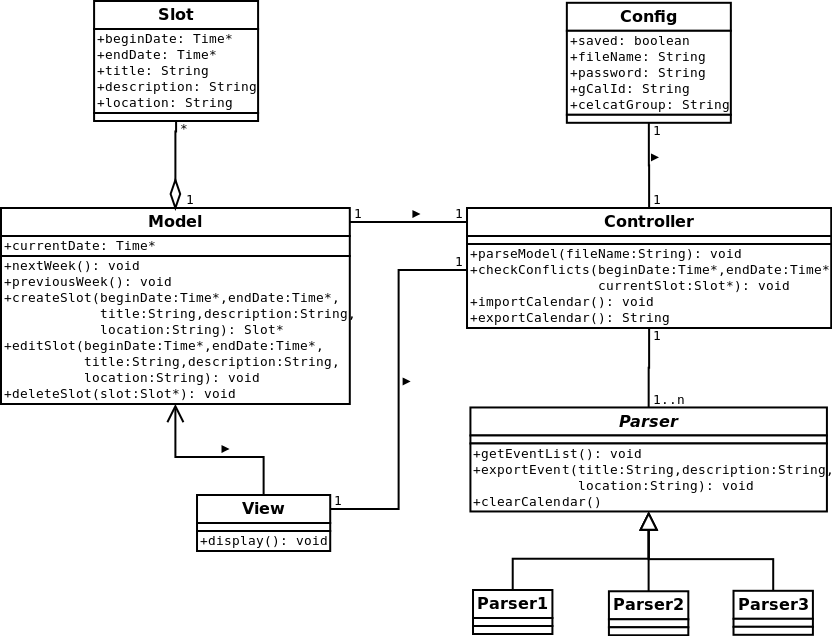
\includegraphics[scale=0.55]{DiagrammeGL.png}
		\caption{Diagramme de classe général}
	\end{figure}
	\FloatBarrier

\chapter{Conception du modèle}
	%JEROME
	
	Le modèle contient toutes les données de l'application, aussi bien les objets de l'emploi du temps manipulés utilisés par les différentes classes que la configuration du logiciel. Il correspond à la première partie du patron architectural MVC. 
	
	Le modèle est composé des classes suivantes :
	\begin{figure}
		\centering
		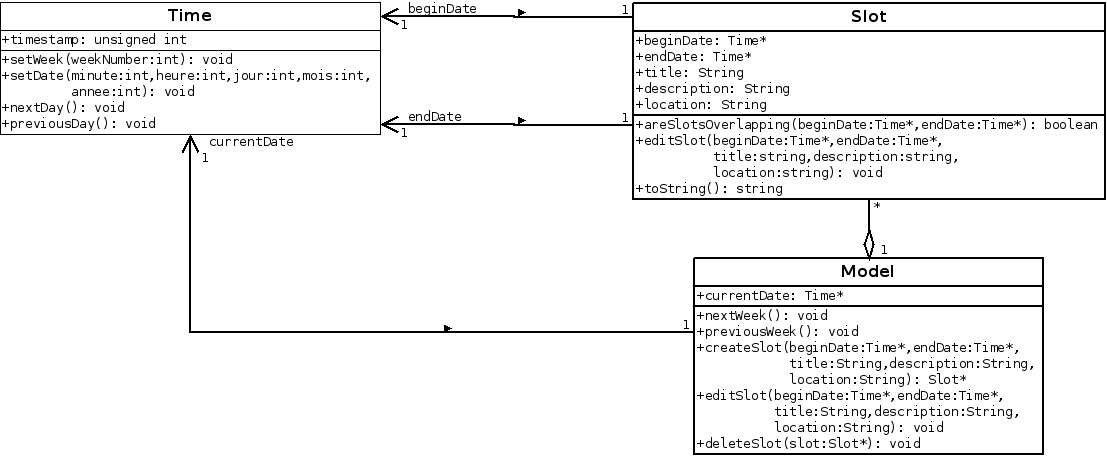
\includegraphics[scale=0.45]{diagclasses_model.png}
		\caption{Diagramme de classe du sous-système \og Model \fg{}}
	\end{figure}
	\FloatBarrier
	
	\section{La classe Modèle}
	La classe modèle est la classe principale de ce sous-système. Elle possède plusieurs types d'attributs :
	\begin{itemize}
		\item Time* currentDate : Un pointeur vers un objet de type Time qui contient la date courante.
        \item Set<Slot*> slotlist : Un ensemble de pointeurs de slot contenu dans un Set afin de trier les objets. De cette manière, les opérations de base (ajout, suppression, lecture et mise à jour) sont disponibles facilement, en parcourant la liste via un itérateur. Pour cela, il sera convenu de définir une méthode de comparaison des créneaux qui se basera sur leur date de début pour effectuer ce tri.
	\end{itemize}
	
	Voici la liste des méthode de cette classe :
		\subsection*{nextWeek}
            Méthode : void nextWeek()
			\begin{itemize}
				\item Objectif  : Mettre l'attribut currentDate à la date du premier jour de la semaine suivante.
				\item Pré-condition : /
				\item Post-condition : La nouvelle date correspond à sept jours après l'ancienne.
			\end{itemize}
			
   		\subsection*{nextWeek}
            Méthode : void nextWeek();
			\begin{itemize}
				\item Objectif  : Mettre l'attribut currentDate à la date du premier jour de la semaine précédente.
				\item Pré-condition : /
				\item Post-condition : La nouvelle date correspond à sept jours avant l'ancienne.
			\end{itemize}
   		\subsection*{createSlot}
            Méthode : Slot* createSlot(Time *beginDate, Time *endDate, string title, string description, string location)
			\begin{itemize}
				\item Objectif  : Création de l'objet Slot correspondant aux données en entrée et ajout dans l'ensemble de créneaux.
				\item Pré-condition : Les données entrées ont été vérifiées (dates biens formées, dates de début et de fin cohérentes et pas de conflits avec d'autres créneaux).
				\item Post-condition : Le créneau est créé et a été ajouté dans l'ensemble slotlist.
			\end{itemize}
            
   		\subsection*{deleteSlot}
            Méthode : void (Slot deleteSlot *slot)
			\begin{itemize}
				\item Objectif  : Suppression dans l'ensemble du créneau concerné et destruction de l'objet.
				\item Pré-condition : Le créneau existe et est dans la collection slotlist.
				\item Post-condition : L'objet n'est plus référencé dans l'ensemble et a été détruit. Il n'est plus accessible via son pointeur.
			\end{itemize}
            
   		\subsection*{cleanList}
            Méthode : void cleanList()
			\begin{itemize}
				\item Objectif  : Destruction de tous les créneaux de l'ensemble slotlist.
				\item Pré-condition : /
				\item Post-condition : Aucun créneau n'est accessible via les pointeurs et l'ensemble de créneau est vide.
			\end{itemize}
            
            
	\section{La classe Slot}    
	La classe Slot est la classe qui contient les données d'un créneau qui contenu dans le modèle. Elle contient toutes les informations qui les définissent : une plage horaire qui explicite les heures de début et de fin ainsi que le titre, la description et le lieu. 
	\begin{itemize}
		\item Time* beginDate : Heure de début de l'événement.
		\item Time* endDate : Heure de fin de l'événement.
		\item String title : Le titre du créneau sous forme de chaine de caractère (string).
		\item String description : Une chaine de caractère qui contient une courte description du créneau.
		\item String location : L'information sur le lieu de l'événement dans une string.
	\end{itemize}
	
	Pour comparer les différents créneaux, il est nécessaire que les opérateurs de comparaison \og == \fg{}  et \og != \fg{}. Dans le cas de l'égalité, tous les attributs devront être identiques pour renvoyer la valeur booléenne \og vrai \fg{} tandis que dans l'opération d'inégalité, il suffit d'une seule différence pour renvoyer \og vrai \fg{}. De cette manière, tous les traitements sur les créneaux se feront de la manière la plus claire et rapide possible pour ne pas alourdir le code.
	
	Les attributs étants tous modifiables par l'utilisateur, il est nécessaire de prévoir des accesseurs. Ceux-ci seront aussi bien des \textit{getters} que des \textit{setters}, qui premettent respectivement d'accéder à la valeur et de la modifier.
	
	Les autres méthodes de cette classe vont être décris maintenant.
   		\subsection*{areSlotsOverlapping}
            Méthode : bool areSlotsOverlapping(Time* beginDate, Time* endDate)
			\begin{itemize}
				\item Objectif  : Vérifier si deux créneaux sont en conflit pour une même plage horaire.
				\item Pré-condition : /
				\item Post-condition : Retourne la valeur booléenne \og vrai \fg{} si les créneaux ont au moins une minute en commun et faux sinon.
			\end{itemize}

   		\subsection*{editSlot}
            Méthode : void editSlot(Time *beginDate, Time *endDate, string intitule, string description)
			\begin{itemize}
				\item Objectif  : Modifier toutes les valeurs d'un créneau à la fois (date et chaines de caractère).
				\item Pré-condition : Les valeurs d'entrée sont au bon format.
				\item Post-condition : Le créneau possède maintenant les nouvelles valeurs.
			\end{itemize}
			
   		\subsection*{toString}
            Méthode : string toString()
			\begin{itemize}
				\item Objectif  :Retourner une chaine de caractère contenant toutes les informations sur le créneau dans une forme lisible par un humain.
				\item Pré-condition : /
				\item Post-condition : La chaine retournée indique la date de début, de fin et l'intitulé du créneau afin de facilement le distinguer des autres.
			\end{itemize}

	\section{La classe Time}  
        Time est la classe qui gère les dates et les opérations temporelles qui s'appliquent dessus. Elle est notamment utilisée pour stocker l'heure et le jour des dates de début et de fin de créneau. Elle est basée sur le mécanisme d'horodatage (ou \og timestamp \fg{}) pour marquer une date en temps UNIX \footnote{Une explication est disponible à \hyperref[cette adresse]{''https://fr.wikipedia.org/wiki/Horodatage''}.} grâce à un entier non signé.
        
        Dans une applications telle que celle-ci, il est courant de manipuler des dates et d'effectuer des comparaisons, c'est pourquoi il est nécessaire de redéfinir un certain nombre d'opérateurs pour cette classe. Cela concerne la supériorité et l'infériorité, strictes ou non, ainsi que l'égalité et l'inégalité.
        
        Le constructeur doit pouvoir ajouter prendre en entrée des valeurs manipulables aisément par un être humain. Cela doit être donc des références au système de temps international : minute, heure, jour, mois et année. Le programme devra donc gérer la conversion vers le timestamp.
        
        Les méthodes de cette classe seront :
   		\subsection*{editSlot}
            Méthode : void setWeek (int week);
			\begin{itemize}
				\item Objectif : Mettre à jour la valeur du timestamp au premier jour d'une semaine spécifique dont le numéro est passé entre paramètre.
				\item Pré-condition : Le numéro de la semaine doit être compris entre 1 et 52 inclus.
				\item Post-condition : La date correspond maintenant au lundi dont le numéro de la semaine est celui-ci.
			\end{itemize}
			
   		\subsection*{setDate}
            Méthode : void setDate(int minute, int hour, int day, int month, int week)
			\begin{itemize}
				\item Objectif : Mettre à jour un timestamp en re-précisant toutes les valeurs temporelles internationales.
				\item Pré-condition : /
				\item Post-condition : Le timestamp UNIX correspond à la date indiquée en entrée sous forme classique.
			\end{itemize}
			
   		\subsection*{nextDay}
            Méthode : void nextDay()
			\begin{itemize}
				\item Objectif : Récupérer la date du jour suivant celle en cours.
				\item Pré-condition : /
				\item Post-condition : Le nouveau jour a été édité et tiens compte de ces modifications.
			\end{itemize}
			
   		\subsection*{previousDay}
            Méthode : void previousDay()
			\begin{itemize}
				\item Objectif : Récupérer la date du jour précédant celle en cours.
				\item Pré-condition : /
				\item Post-condition : Le nouveau jour a été édité et tiens compte de ces modifications.
        \newline
			\end{itemize}
        En plus de ces opérations, il est nécessaire de proposer des accesseurs pour toutes les unités internationales suivantes : minute, heure, jour, semaine, mois et année. Ainsi, il sera facile d'éditer seulement une seule valeur à la fois.

\chapter{Conception des interfaces de communication}
	%GUILLAUME
	Ce sous-système de l'application MyCalendar constitue, derrière le modèle local, son centre névralgique. En effet, c'est toute cette partie de l'application qui va gérer les communications avec l'extérieur, que ce soit pour récupérer un calendrier distant ou pour exporter en ligne les données locales.\\
	
	Il existe deux types de communications : les communications entrantes (import d'un calendrier vers les données locales) et les communications sortantes (export des données locales vers un calendrier distant).
	
	Premièrement, l'application est sensée, à terme, pouvoir gérer plusieurs types de services en ligne. Cela signifie qu'il faut non seulement permettre aux développeur de pouvoir ajouter la prise en charge d'un nouveau service facilement, mais aussi proposer aux utilisateurs une interface lui proposant de choisir lui-même quel service il souhaite utiliser pour l'import comme pour l'export.
	
	Deuxièmement, un service de calendrier propose l'import de données en même temps que l'export de données. Cela ne sera pas vrai pour un emploi du temps universitaire, qui est sensé ne pas pouvoir être modifiable par un client quelconque, mais cela le sera normalement pour tout autre service distant.
	
	Partant de ces deux conclusions, nous avons décidé de partir sur la conception d'une classe abstraite \emph{Parser} déclarant toutes les méthodes permettant l'import et l'export de données. Pour implémenter un nouveau service distant, il faut ensutie étendre cette classe abstraite et de définir les méthodes qu'il faut. Enfin, pour l'utiliser, il suffira de modifier le controller (que nous avons vu précédemment) pour instancier ce parseur et utiliser les méthodes que l'ont veut.\\
	
	Dans l'application \emph{MyCalendar}, seulement deux parseurs ont été définis.
	\begin{figure}
		\centering
		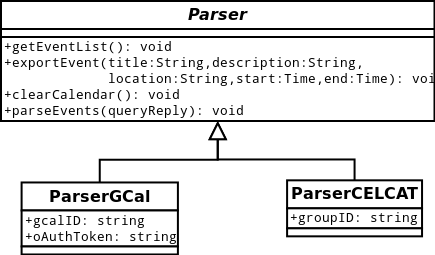
\includegraphics[scale=0.65]{diagclasses_parser.png}
		\caption{Diagramme de classe des interfaces de communication}
	\end{figure}
	\FloatBarrier

\chapter{Conception de l'interface utilisateur}
	%JEROME

